\chapter*{\fontb EXAMPLE\\}
\toca{chapter}{\fonta{14}}{EXAMPLE}

\tocb{section}{12}{Creating mini-pages}

%use of \\ at the end of the line changes the paragraph
Use 2 backslashes ($\backslash\backslash$) and the end to line to change
the paraghraph\\

This is an example for writing 2 paragraph side by side\textbf{:}\\

\begin{minipage}{0.45\textwidth} %minipage width is 49% of textwidth
Lorem ipsum dolor sit amet, consectetur adipiscing elit. Mauris vitae viverra
felis. Pellentesque dui sapien, ullamcorper vel justo vestibulum, molestie
ultricies mauris. Donec nec nunc ullamcorper, suscipit tortor sed, hendrerit
\end{minipage}
\hspace{0.5cm} %horizontal space of 0.5 cm
\begin{minipage}{0.45\textwidth}
dapibus nibh tincidunt nec. Sed aliquet nisl at diam pharetra, et volutpat dui
dictum. Vestibulum condimentum, leo eget vestibulum vestibulum, turpis sem
tempor ante, id rutrum orci elit sed diam. Mauris mattis justo ut erat
\end{minipage}

\vspace{0.5cm} %vertical space of 0.5 cm
This is an example for writing 3 paragraph side by side\textbf{:}\\

\begin{minipage}{0.30\textwidth}
Curabitur mi diam, sagittis sed laoreet eu, lacinia vel augue. Quisque pretium
nunc a mauris semper accumsan et at nisl. Vestibulum vitae commodo erat, non
tristique leo. Ut non semper libero. Cras luctus orci ut eros egestas, quis
\end{minipage}
\hspace{0.5cm}
\begin{minipage}{0.30\textwidth}
elementum urna. Suspendisse accumsan finibus odio posuere facilisis. Sed
cursus, lectus elementum fringilla auctor, justo quam lacinia erat, ac blandit
nunc arcu in lorem. Nunc nec pulvinar lacus. Vivamus tristique imperdiet ipsum,
\end{minipage}
\hspace{0.5cm}
\begin{minipage}{0.30\textwidth}
urna molestie, nec molestie elit suscipit. Duis fringilla leo fringilla enim
pulvinar, ut rutrum orci tincidunt. Morbi scelerisque est at eros lobortis
luctus. Ut ipsum nisl, faucibus quis ultricies eget, rhoncus et nulla.
\end{minipage}\\

\tocb{section}{12}{Inserting images}

This is an example of insterting graphics.

\begin{figure}[H]
	\centering
	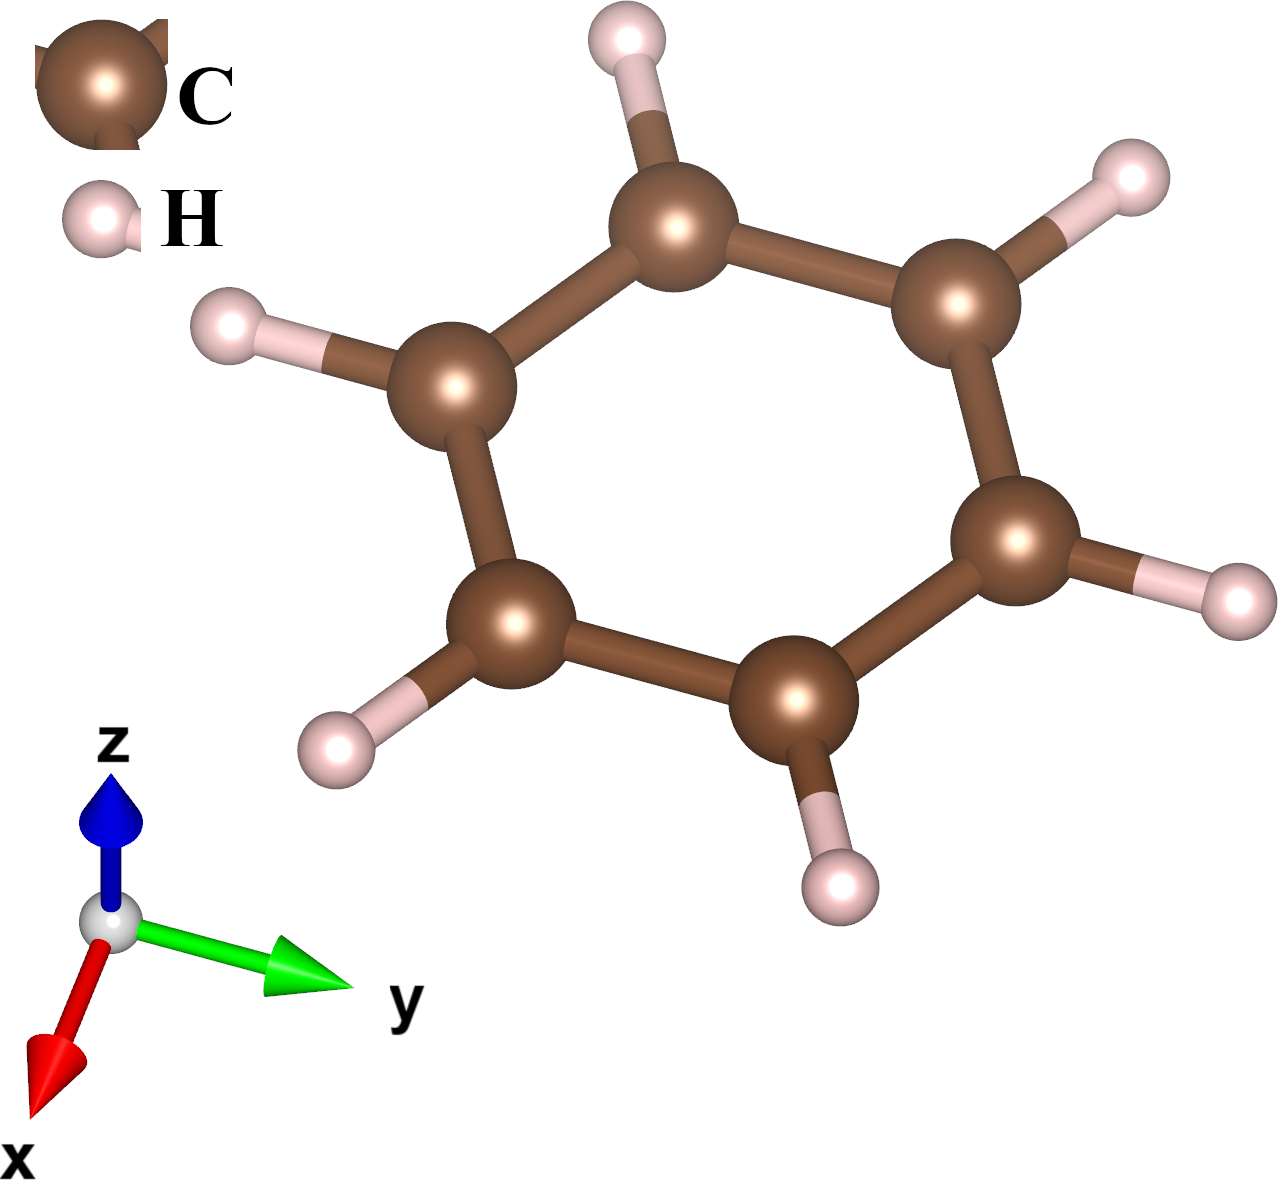
\includegraphics[width=5cm]{Benzene}
	%caption written between [ ] is shown in list of figure and caption
	%written between { } is shown just below the figure in the page
	\caption[C\tsb{6}H\tsb{6} structure]{Structure of Benzene (Created using
	VESTA \&\ edited with GIMP)}
	%add any unique variable between { } to use while refrencing
	\label{fig:benzene}
\end{figure}

This is an example of insterting multiple images in same line.

\begin{figure}[H]
	\centering
	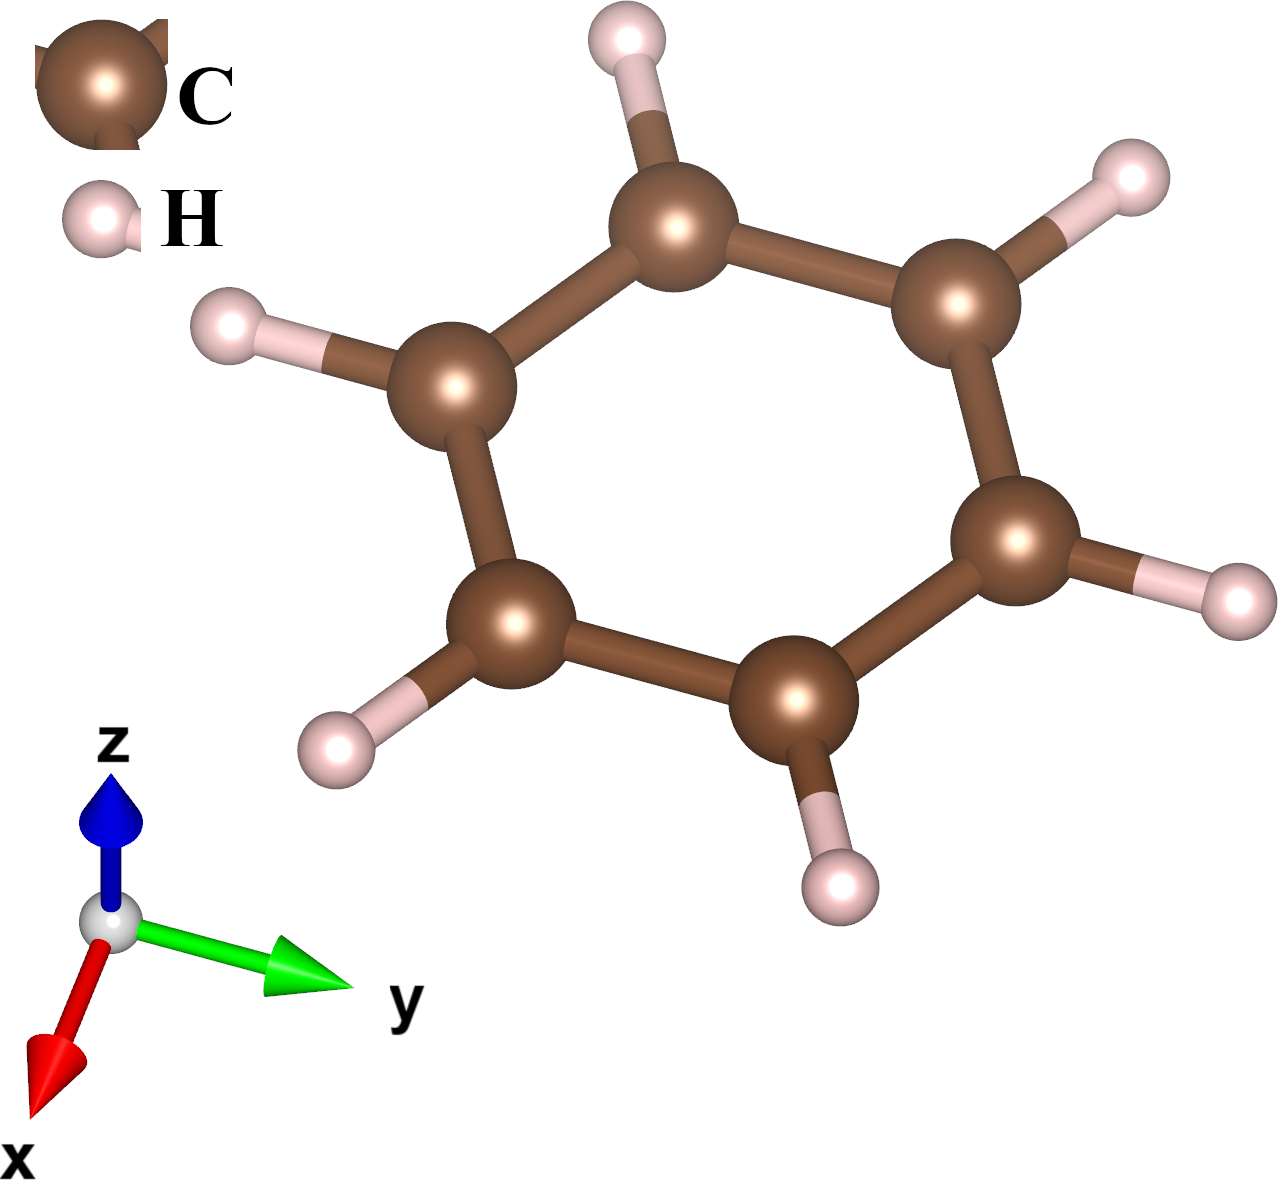
\includegraphics[width=5cm]{Benzene}
	\hspace{0.5cm}
	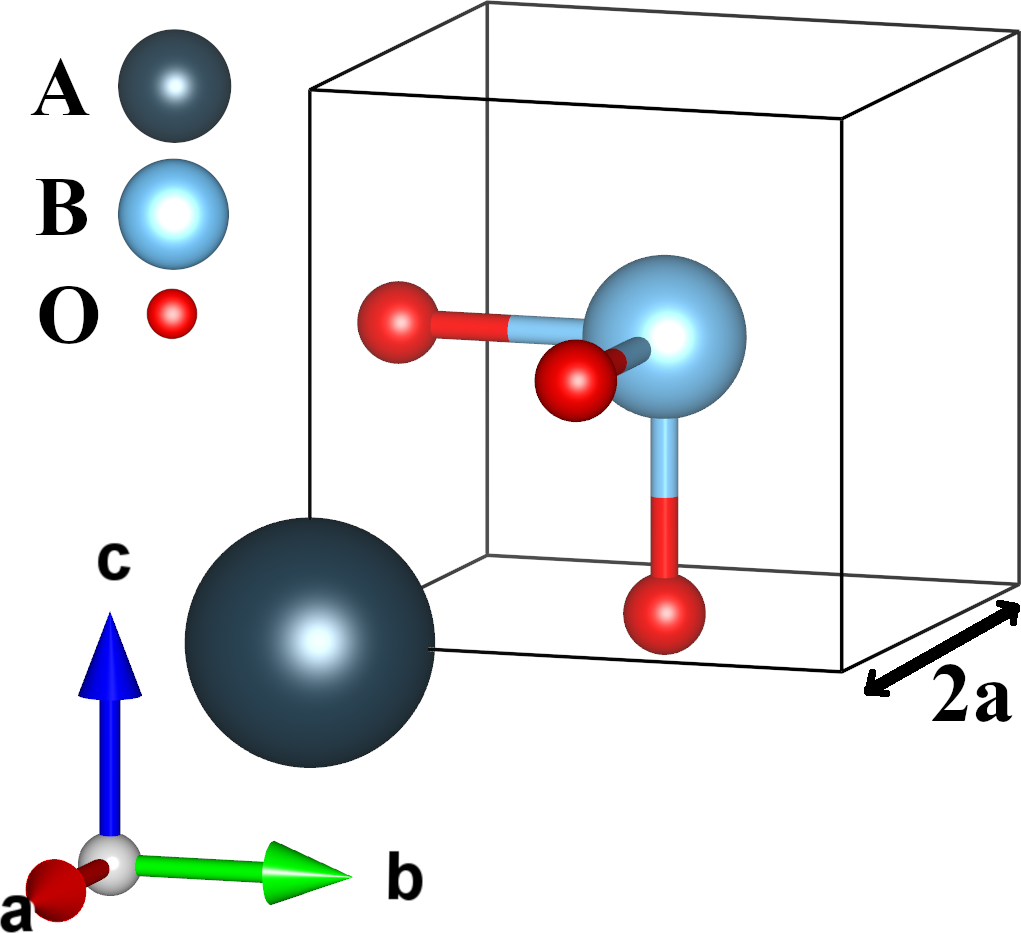
\includegraphics[width=5cm]{perovskite_unitcell}
	\caption[C\tsb{6}H\tsb{6} \&\ ABO\tsb{3} structure]{Structure of Benzene
	and Unit cell of perovskite (Created using VESTA \&\ edited with GIMP)}
\end{figure}

\tocb{section}{12}{Inserting tables}

This is an example of insterting table.

\begin{table}[H] %[H] prints the table right at this position
	\centering
% | wtill vetical line separeting columns
% c means the component of the cell is centered 
\begin{tabular}{|c|c|c|c|}
	\hline %creates horizontal bar
	% & seperates the each componets of the cell
	Atoms & x & y & z\\ % \\ ends the row and start new row
	\hline
	A & 0.25 & 0.25 & 0.25\\
	% here we havent written hline so horizontal line wont show in table 
	B & 0.25 & 0.00 & 0.00\\
	C & 0.00 & 0.00 & 0.00\\
	D & 0.50 & 0.00 & 0.00\\
	\hline
\end{tabular}
	\caption[Atomic coordinates 1]{Atomic coordinates 1}
	\label{tab:atom}
\end{table}

This is an example of combining multiple column or multiple row in a table.

\begin{table}[H]
	\centering
\begin{tabular}{|c|c|c|c|}
	\hline
	% {2} represents merging ot 2 column in that row, {c|} mean center align
	Atoms & x & \multicolumn{2}{c|}{y \&\ z}\\
	\hline
	A  & 0.25 & 0.25 & 0.25\\
	\cline{2-4} % creates horizontal line from column 2 to 4
	{} & 0.25 & 0.00 & 0.00\\ % {} at the begining represents cell in empty
	\hline
	C  & 0.00 & 0.00 & 0.00\\
	\hline
	D  & 0.50 & 0.00 & 0.00\\
	\hline
\end{tabular}
	\caption[Atomic coordinates 2]{Atomic coordinates 2}
\end{table}

\tocb{section}{12}{Writing equations}

This is an example for lengthy equation which doesn't fit in one line.
Use multline environment for this.

%add \\ where you want to break the equation and start from second line
\begin{multline}
	e^x = 1+x+\frac{x^2}{2!}+\frac{x^3}{3!}+\frac{x^4}{4!}+\frac{x^5}{5!}
	+\frac{x^6}{6!}+\frac{x^7}{7!}\\+\frac{x^8}{8!}+\frac{x^9}{9!}
	+\frac{x^{10}}{10!}+\frac{x^{11}}{11!}+\frac{x^{12}}{12!}
	+\frac{x^{13}}{13!}+\frac{x^{14}}{14!}+\cdots
	\label{eq:expansion}
\end{multline}

This is an example for writing multiple equations at a time.
Use align environment for this.

\begin{align}
	2x+6y&=64\\
	x+3y&=32
	\label{eq:xy}
\end{align}

\tocb{section}{12}{Referencing}

You can the bibtex citation key to put in reference.bib file in the site
Google Scholar.\\

Cite website and application like this: \hspace{1cm}
%put the variable from rerefence.bib file inbetween the { }
\cite{williams_gnuplot_nodate}

Cite articles and books like this: \hspace{1cm}
\cite{hohenberg1964inhomogeneous}

You can also put it inside square brackets like this: \hspace{1cm}
[\cite{hohenberg1964inhomogeneous}]   \\

You also can reference tables like this: \hspace{1cm} 
%put the variable you used in label inbetween \ref{ }
\textbf{Table \ref{tab:atom}}


You also can reference figure like this: \hspace{1cm} 
%put the variable you used in label inbetween \ref{ }
\textbf{Figure \ref{fig:benzene}}


You also can reference equations like this: \hspace{1cm} 
%put the variable you used in label inbetween \ref{ }
\textbf{Equation \ref{eq:expansion}}




















